% answers.tex —— 1977 年·福建卷·理科 · 参考答案与详细解析片段
% 由 tools/generate_projects.py 依来源总账自 1977/1977_数学真题_福建理_试题.md + 1977/1977_数学真题_福建理_解析正文.md + 1977/1977_数学真题_福建理_答案要点.md 生成，勿手改（改源 MD 后重跑）


\begin{gktip}
固定源为 A3 单页题面，未附答案页。第 1 题含十个小问，正式题为第 1—7 题，附加题 8、9 保留在第 7 题之后。第 5、第 6、第 7 的源面参数或条件存在已登记问题，以下严格区分按字面结论与待核说明。
\end{gktip}

\begin{answer}
\gksolhead{1}{}

\textbf{题目}：

\Needspace{5\baselineskip}
（1） 计算：

\nopagebreak[4]
\[
5-3\times\left[\left(-3\frac38\right)^{-\frac13}+1031\times\left(0.25-2^{-2}\right)\right]\div9^0
\]

\Needspace{5\baselineskip}
（2） 求下列式子的正负：

\nopagebreak[4]
\[
y=\frac{\cos160^\circ-\cos170^\circ}{\tan155^\circ}
\]

的值是正的还是负的？为什么？

\Needspace{5\baselineskip}
（3） 求函数

\nopagebreak[4]
\[
y=\frac{\lg(2-x)}{\sqrt{x}-1}
\]

的定义域。

（4） 如图，在梯形 $ABCD$ 中，$DM=MP=PA$，$MN\parallel PQ\parallel AB$，$DC=2\ \mathrm{cm}$，$AB=3.5\ \mathrm{cm}$，求 $MN$ 和 $PQ$ 的长。
\nopagebreak[4]
\begin{center}% 1977 年福建卷理科第 1(4) 题：梯形三等分平行线
\begin{tikzpicture}[scale=0.78]
  \coordinate (D) at (1.0,4.2);
  \coordinate (C) at (4.8,4.2);
  \coordinate (A) at (0,0);
  \coordinate (B) at (5.8,0);
  \coordinate (M) at ($(D)!1/3!(A)$);
  \coordinate (N) at ($(C)!1/3!(B)$);
  \coordinate (P) at ($(D)!2/3!(A)$);
  \coordinate (Q) at ($(C)!2/3!(B)$);
  \draw[thick] (D)--(C)--(B)--(A)--cycle;
  \draw[thick] (M)--(N);
  \draw[thick] (P)--(Q);
  \node[above left] at (D) {$D$};
  \node[above right] at (C) {$C$};
  \node[below left] at (A) {$A$};
  \node[below right] at (B) {$B$};
  \node[left] at (M) {$M$};
  \node[right] at (N) {$N$};
  \node[left] at (P) {$P$};
  \node[right] at (Q) {$Q$};
  \node[above] at (2.9,4.2) {$2$};
  \node[below] at (2.9,0) {$3.5$};
\end{tikzpicture}
\end{center}
\nopagebreak[4]
（5） 已知 $\lg3=0.4771$，$\lg x=-3.5229$，求 $x$。

\Needspace{5\baselineskip}
（6） 求

\nopagebreak[4]
\[
\lim_{x\to1}\frac{x-1}{x^2-3x+2}
\]

\Needspace{5\baselineskip}
（7） 解方程：

\nopagebreak[4]
\[
\sqrt{4x+1}-2x+1=0
\]

\Needspace{5\baselineskip}
（8） 化简：

\nopagebreak[4]
\[
\frac{a^{2n+1}-6a^{2n}+9a^{2n-1}}{a^{n+1}-4a^n+3a^{n-1}}
\]

（9） 求函数 $y=2-5x-3x^2$ 的极值。

（10） 画出下面 $V$ 形铁块的三视图（只要画草图）。
\nopagebreak[4]
\begin{center}% 1977 年福建卷理科第 1(10) 题：V 形铁块示意图
% 源卷只要求据图画三视图，未给尺寸；此处重绘结构关系，不虚构尺寸。
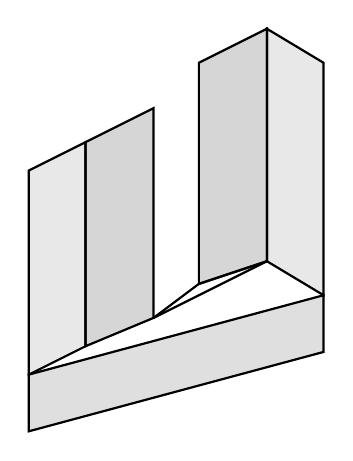
\begin{tikzpicture}[scale=0.72]
  \fill[gray!25] (0,0)--(5.2,1.4)--(5.2,2.4)--(0,1.0)--cycle;
  \draw[thick] (0,0)--(5.2,1.4)--(5.2,2.4)--(0,1.0)--cycle;
  \fill[gray!18] (0,1.0)--(0,4.6)--(1.0,5.1)--(1.0,1.5)--cycle;
  \fill[gray!32] (1.0,1.5)--(1.0,5.1)--(2.2,5.7)--(2.2,2.0)--cycle;
  \draw[thick] (0,1.0)--(0,4.6)--(1.0,5.1)--(1.0,1.5)--cycle;
  \draw[thick] (1.0,1.5)--(1.0,5.1)--(2.2,5.7)--(2.2,2.0)--cycle;
  \fill[gray!18] (5.2,2.4)--(5.2,6.5)--(4.2,7.1)--(4.2,3.0)--cycle;
  \fill[gray!32] (4.2,3.0)--(4.2,7.1)--(3.0,6.5)--(3.0,2.6)--cycle;
  \draw[thick] (5.2,2.4)--(5.2,6.5)--(4.2,7.1)--(4.2,3.0)--cycle;
  \draw[thick] (4.2,3.0)--(4.2,7.1)--(3.0,6.5)--(3.0,2.6)--cycle;
  \draw[thick] (2.2,2.0)--(3.0,2.6);
  \draw[thick] (2.2,2.0)--(4.2,3.0);
  \draw[thick] (3.0,2.6)--(4.2,3.0);
  \draw[dashed] (2.2,2.0)--(2.2,5.7);
  \draw[dashed] (3.0,2.6)--(3.0,6.5);
\end{tikzpicture}
\end{center}
\nopagebreak[4]
\Needspace{4\baselineskip}
\textbf{解析}

\gksubpart{（1）}

\Needspace{5\baselineskip}
因为 $-3\frac38=-\frac{27}{8}$，且

\nopagebreak[4]
\[
\left(-\frac{27}{8}\right)^{-\frac13}=-\frac23,
\qquad
0.25-2^{-2}=0,
\qquad
9^0=1
\]

\Needspace{5\baselineskip}
所以

\nopagebreak[4]
\[
5-3\left(-\frac23+1031\times0\right)\div1=7
\]

\gksubpart{（2）}

\Needspace{5\baselineskip}
在 $0^\circ$ 到 $180^\circ$ 上余弦函数递减，故 $160^\circ<170^\circ$ 时

\nopagebreak[4]
\[
\cos160^\circ-\cos170^\circ>0
\]

而 $\tan155^\circ=-\tan25^\circ<0$，因此原分式的值为负。

\gksubpart{（3）}

\Needspace{5\baselineskip}
对数真数要求 $2-x>0$，根式要求 $x\ge0$，分母还要求 $\sqrt{x}-1\ne0$，即 $x\ne1$。所以定义域为

\nopagebreak[4]
\[
[0,1)\cup(1,2)
\]

\gksubpart{（4）}

\Needspace{5\baselineskip}
由 $DM=MP=PA$，侧边从 $D$ 到 $A$ 被三等分。平行截线长度沿侧边作线性变化，因此

\nopagebreak[4]
\[
MN=DC+\frac13(AB-DC)=2+\frac13(3.5-2)=2.5\ \mathrm{cm}
\]

\Needspace{5\baselineskip}
以及

\nopagebreak[4]
\[
PQ=DC+\frac23(AB-DC)=2+\frac23(3.5-2)=3\ \mathrm{cm}
\]

\gksubpart{（5）}

\nopagebreak[4]
\[
\lg x=-3.5229=0.4771-4=\lg3-\lg10^4=\lg(3\times10^{-4})
\]

故 $x=0.0003$。

\gksubpart{（6）}

\nopagebreak[4]
\[
\lim_{x\to1}\frac{x-1}{x^2-3x+2}
=\lim_{x\to1}\frac{x-1}{(x-1)(x-2)}
=\lim_{x\to1}\frac1{x-2}=-1
\]

\gksubpart{（7）}

\Needspace{5\baselineskip}
根式方程要求 $4x+1\ge0$，且移项后 $\sqrt{4x+1}=2x-1$ 要求 $x\ge1/2$。平方得

\nopagebreak[4]
\[
4x+1=(2x-1)^2
\quad\Longleftrightarrow\quad
4x(x-2)=0
\]

候选 $x=0,2$ 中只有 $x=2$ 满足 $x\ge1/2$，故 $x=2$。

\gksubpart{（8）}

\Needspace{5\baselineskip}
分子、分母分别提取幂因子：

\nopagebreak[4]
\[
\begin{aligned}
\frac{a^{2n+1}-6a^{2n}+9a^{2n-1}}
{a^{n+1}-4a^n+3a^{n-1}}
&=\frac{a^{2n-1}(a-3)^2}{a^{n-1}(a-1)(a-3)}\\
&=\frac{a^n(a-3)}{a-1}
\end{aligned}
\]

上式只在原分式有意义且约分合法时成立；至少需要排除使原分母为零的情形，不能把约分结果当作全体 $a,n$ 的定义域。

\gksubpart{（9）}

\nopagebreak[4]
\[
y=2-5x-3x^2=-3\left(x+\frac56\right)^2+\frac{49}{12}
\]

所以函数在 $x=-5/6$ 时取得最大值 $49/12$。

\gksubpart{（10）}

源题只要求根据所示 V 形铁块画三视图草图，没有给出尺寸。项目中以 TikZ 重绘源图的结构示意，供三视图作图时辨认形体；不据无尺寸图形虚构唯一的三视图尺寸答案。

\gkanswer{答案（1）：$7$。}

\gkanswer{答案（2）：负。}

\gkanswer{答案（3）：$[0,1)\cup(1,2)$。}

\gkanswer{答案（4）：$MN=2.5\ \mathrm{cm}$，$PQ=3\ \mathrm{cm}$。}

\gkanswer{答案（5）：$x=0.0003$。}

\gkanswer{答案（6）：$-1$。}

\gkanswer{答案（7）：$x=2$。}

\gkanswer{答案（8）：$\dfrac{a^n(a-3)}{a-1}$（在原式有意义的条件下）。}

\gkanswer{答案（9）：最大值为 $\dfrac{49}{12}$，在 $x=-\dfrac56$ 时取得。}

\gkanswer{答案（10）：见解析版；按源卷所示 V 形铁块作三视图草图。}

\end{answer}
\begin{answer}
\gksolhead{2}{}

\textbf{题目}：

\Needspace{5\baselineskip}
（1） 解不等式：

\nopagebreak[4]
\[
\frac{x^2-x-6}{x^2+2x+2}<0
\]

\Needspace{5\baselineskip}
（2） 证明：

\nopagebreak[4]
\[
\frac{2\cos\theta-\sin2\theta}{2\cos\theta+\sin2\theta}
=\tan^2\left(\frac{90^\circ-\theta}{2}\right)
\]

（3） 某中学革命师生自己动手油漆一个直径为 $1.2\ \mathrm m$ 的地球仪，如果每平方米面积需要油漆 $150$ 克，问共需油漆多少克？（答案保留整数。）

（4） 某农机厂开展“工业学大庆”运动，在十月份生产拖拉机 $1000$ 台。这样，一月至十月的产量恰好完成全年生产任务。工人同志为了加速农业机械化，计划在年底前再生产 $2310$ 台，求十一月、十二月份平均每月增长率。

\Needspace{4\baselineskip}
\textbf{解析}

\gksubpart{（1）}

\Needspace{5\baselineskip}
因为 $x^2+2x+2=(x+1)^2+1>0$ 对一切实数 $x$ 成立，所以只需解

\nopagebreak[4]
\[
x^2-x-6=(x-3)(x+2)<0
\]

\Needspace{5\baselineskip}
故解集为

\nopagebreak[4]
\[
-2<x<3
\]

\gksubpart{（2）}

\Needspace{5\baselineskip}
在分母有意义且不为零的范围内，利用 $\sin2\theta=2\sin\theta\cos\theta$：

\nopagebreak[4]
\[
\begin{aligned}
\frac{2\cos\theta-\sin2\theta}{2\cos\theta+\sin2\theta}
&=\frac{2\cos\theta(1-\sin\theta)}{2\cos\theta(1+\sin\theta)}\\
&=\frac{1-\sin\theta}{1+\sin\theta}
=\tan^2\left(\frac{90^\circ-\theta}{2}\right)
\end{aligned}
\]

\gksubpart{（3）}

\Needspace{5\baselineskip}
地球仪视为球体，半径为 $0.6\ \mathrm m$，表面积为

\nopagebreak[4]
\[
4\pi(0.6)^2=1.44\pi\ \mathrm{m^2}
\]

\Needspace{5\baselineskip}
所需油漆质量为

\nopagebreak[4]
\[
150\times1.44\pi=216\pi\ \mathrm g\approx678.24\ \mathrm g
\]

保留整数得 $678\ \mathrm g$（取 $\pi=3.14$）。

\gksubpart{（4）}

\Needspace{5\baselineskip}
若按题意把十一、十二月理解为从十月的 $1000$ 台按相同月增长率递增，设增长因子为 $q=1+r$，则

\nopagebreak[4]
\[
1000q+1000q^2=2310
\quad\Longleftrightarrow\quad
q^2+q-2.31=0
\]

\Needspace{5\baselineskip}
正的增长因子为 $q=1.1$，故平均每月增长率的候选值为

\nopagebreak[4]
\[
r=10\%
\]

\gkanswer{答案（1）：$-2<x<3$。}

\gkanswer{答案（2）：见解析版。}

\gkanswer{答案（3）：$216\pi\ \mathrm g\approx678\ \mathrm g$（取 $\pi=3.14$）。}

\gkanswer{答案（4）：在十一、十二月从十月产量按同一增长率递增的解释下，平均每月增长率为 $10\%$。}

\end{answer}
\begin{answer}
\gksolhead{3}{}

\textbf{题目}：

在半径为 $R$ 的圆内接正六边形内，依次连接各边的中点，得一正六边形；又在这一正六边形内，再依次连接各边的中点，又得一正六边形，这样无限地继续下去，求：

（1） 前 $n$ 个正六边形的周长之和 $S_n$；

（2） 所有这些正六边形的周长之和 $S$。

\Needspace{4\baselineskip}
\textbf{解析}

\Needspace{5\baselineskip}
设第 $k$ 个正六边形的外接圆半径为 $R_k$。正六边形边长等于外接圆半径，连接各边中点后，新正六边形的外接圆半径等于原六边形的内切圆半径，因此

\nopagebreak[4]
\[
R_{k+1}=\frac{\sqrt3}{2}R_k
\]

令 $q=\sqrt3/2$，则第 $k$ 个正六边形的周长为 $6Rq^{k-1}$。

\gksubpart{（1）}

\Needspace{5\baselineskip}
前 $n$ 个正六边形的周长之和为

\nopagebreak[4]
\[
S_n=6R\frac{1-q^n}{1-q}
\]

\gksubpart{（2）}

\Needspace{5\baselineskip}
由于 $0<q<1$，所有正六边形的周长之和为

\nopagebreak[4]
\[
S=\frac{6R}{1-q}
=\frac{6R}{1-\sqrt3/2}
=12R(2+\sqrt3)
\]

\gkanswer{答案（1）：令 $q=\dfrac{\sqrt3}{2}$，则 $S_n=6R\dfrac{1-q^n}{1-q}$。}

\gkanswer{答案（2）：$S=\dfrac{6R}{1-q}=12R(2+\sqrt3)$。}

\end{answer}
\begin{answer}
\gksolhead{4}{}

\textbf{题目}：

动点 $P(x,y)$ 到两定点 $A(-3,0)$ 和 $B(3,0)$ 的距离的比等于 $2$，求动点 $P$ 的轨迹方程，并说明这轨迹是什么图形。

\Needspace{4\baselineskip}
\textbf{解析}

\Needspace{5\baselineskip}
距离比为 $2$ 给出

\nopagebreak[4]
\[
\sqrt{(x+3)^2+y^2}=2\sqrt{(x-3)^2+y^2}
\]

\Needspace{5\baselineskip}
平方并整理：

\nopagebreak[4]
\[
x^2+6x+9+y^2=4x^2-24x+36+4y^2
\]

\Needspace{5\baselineskip}
即

\nopagebreak[4]
\[
(x-5)^2+y^2=16
\]

所以轨迹为圆，圆心为 $(5,0)$，半径为 $4$。

\gkanswer{答案：$(x-5)^2+y^2=16$，为圆，圆心 $(5,0)$、半径 $4$。}

\end{answer}
\begin{answer}
\gksolhead{5}{}

\textbf{题目}：

某大队在农田基本建设的规划中，要测定被障碍物隔开的两点 $A\text{、}P$ 之间的距离，他们土法上马，在障碍物的两侧选取两点 $B$ 和 $C$（如图），测得 $AB=AC=50\ \mathrm m$，$\angle BAC=60^\circ$，$\angle ABP=120^\circ$，$\angle ACP=135^\circ$，求 $A$ 和 $P$ 之间的距离。（答案可用最简根式表示。）
\nopagebreak[4]
\begin{center}% 1977 年福建卷理科第 5 题：障碍物两侧测距示意图
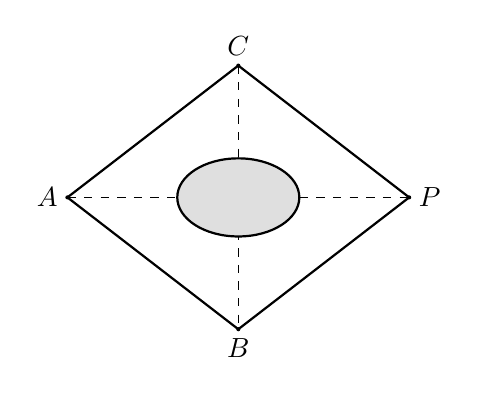
\begin{tikzpicture}[scale=0.62]
  \coordinate (A) at (0,0);
  \coordinate (P) at (7.0,0);
  \coordinate (C) at (3.5,2.7);
  \coordinate (B) at (3.5,-2.7);
  \draw[thick] (A)--(C)--(P)--(B)--cycle;
  \draw[dashed] (A)--(P);
  \draw[dashed] (C)--(B);
  \fill[gray!25] (3.5,0) ellipse (1.25 and 0.8);
  \draw[thick] (3.5,0) ellipse (1.25 and 0.8);
  \fill (A) circle (1.2pt) node[left] {$A$};
  \fill (P) circle (1.2pt) node[right] {$P$};
  \fill (C) circle (1.2pt) node[above] {$C$};
  \fill (B) circle (1.2pt) node[below] {$B$};
\end{tikzpicture}
\end{center}
\nopagebreak[4]
\Needspace{4\baselineskip}
\textbf{解析}

\Needspace{5\baselineskip}
由 $AB=AC=50$ 且 $\angle BAC=60^\circ$，$\triangle ABC$ 为等边三角形。取

\nopagebreak[4]
\[
A=(0,0),\quad B=(25,-25\sqrt3),\quad C=(25,25\sqrt3)
\]

则从 $B$ 出发与 $BA$ 成普通角 $120^\circ$ 的射线方向只能为 $0^\circ$ 或 $240^\circ$；从 $C$ 出发与 $CA$ 成普通角 $135^\circ$ 的射线方向只能为 $15^\circ$ 或 $105^\circ$。前一组射线的纵坐标不大于 $-25\sqrt3$，后一组射线的纵坐标不小于 $25\sqrt3$，四种组合均不能相交于图示同一点 $P$。

因此当前固定源在普通平面角定义下条件不相容，不能可靠给出 $AP$ 的唯一长度；需要权威题面或勘误确认。

\gkanswer{答案：按普通平面角定义，$AB=AC$ 且 $\angle BAC=60^\circ$ 与 $\angle ABP=120^\circ$、$\angle ACP=135^\circ$ 不相容，当前源面无法给出可靠唯一的 $AP$。}

\end{answer}
\begin{answer}
\gksolhead{6}{}

\textbf{题目}：

\Needspace{5\baselineskip}
已知双曲线

\nopagebreak[4]
\[
\frac{x^2}{24\alpha}-\frac{y^2}{16\cot\alpha}=1\quad(\alpha\text{ \text{为锐角}})
\]

和圆 $(x-m)^2+y^2=r^2$ 相切于点 $A(4\sqrt3,4)$，求 $\alpha\text{、}m\text{、}r$ 的值。

\Needspace{4\baselineskip}
\textbf{解析}

\Needspace{5\baselineskip}
将 $A=(4\sqrt3,4)$ 代入源面双曲线，得

\nopagebreak[4]
\[
\frac{48}{24\alpha}-\frac{16}{16\cot\alpha}=1
\quad\Longleftrightarrow\quad
\frac2\alpha-\tan\alpha=1
\]

\Needspace{5\baselineskip}
若把 $\alpha$ 按弧度数处理，锐角数值根约为

\nopagebreak[4]
\[
\alpha=0.8924934\ \mathrm{rad}=51.1361^\circ
\]

\Needspace{5\baselineskip}
双曲线在 $A$ 点的切线斜率为

\nopagebreak[4]
\[
k_h=\frac{2x\cot\alpha}{3\alpha y}
=\frac{2\sqrt3\cot\alpha}{3\alpha}
\]

\Needspace{5\baselineskip}
圆心为 $(m,0)$ 的圆在 $A$ 点的切线斜率为 $-(4\sqrt3-m)/4$，所以

\nopagebreak[4]
\[
m=4\sqrt3+\frac{8\sqrt3\cot\alpha}{3\alpha},
\qquad
r=\sqrt{(4\sqrt3-m)^2+16}
\]

按上述弧度候选根计算，得到 $m\approx11.0987$、$r\approx5.7786$。因源式参数形式异常且没有答案页，这些只能作为按字面解释的候选值。

\gkanswer{答案：按源式可列 $\dfrac2\alpha-\tan\alpha=1$；若按弧度取锐角数值根，则 $\alpha\approx51.1361^\circ$，$m\approx11.0987$，$r\approx5.7786$，仅作按字面解释的候选。}

\end{answer}
\begin{answer}
\gksolhead{7}{}

\textbf{题目}：

\Needspace{5\baselineskip}
设数列 $1,2,4,\ldots$ 前 $n$ 项和是

\nopagebreak[4]
\[
S_n=a+bn+cn^2+dn^3
\]

求这数列的通项 $a_n$ 的公式，并确定 $a,b,c,d$ 的值。

\begin{gktip}
\Needspace{0.25\textheight}
\textbf{附加题}
\end{gktip}

\Needspace{5\baselineskip}
\textbf{附加题 8．} 求函数

\nopagebreak[4]
\[
y=\mathrm e^{-2x}\sin\left(5x+\frac\pi4\right)
\]

的导数。

\Needspace{5\baselineskip}
\textbf{附加题 9．} 求定积分：

\nopagebreak[4]
\[
\int_0^1\left(x\mathrm e^{x^2}+x^2\mathrm e^{2x}\right)\,\mathrm dx
\]

\Needspace{4\baselineskip}
\textbf{解析}

\Needspace{5\baselineskip}
若数列确为 $1,2,4,\ldots$，则其前 $n$ 项和应为

\nopagebreak[4]
\[
S_n=1+2+\cdots+2^{n-1}=2^n-1
\]

\Needspace{5\baselineskip}
这不可能对所有 $n$ 同时等于三次多项式 $a+bn+cn^2+dn^3$。例如由 $S_0=0,S_1=1,S_2=3,S_3=7$ 拟合可得

\nopagebreak[4]
\[
a=0,\qquad b=\frac56,\qquad c=0,\qquad d=\frac16
\]

但该多项式给出 $S_4=14$，而数列实际前四项和为 $15$。因此源题面条件矛盾，不能可靠确定所要求的 $a,b,c,d$。

\gksubpart{附加题 8}

\Needspace{4\baselineskip}
\textbf{解析}

\Needspace{5\baselineskip}
令 $u=5x+\pi/4$，由乘积求导法则

\nopagebreak[4]
\[
y'=\mathrm e^{-2x}\left[5\cos\left(5x+\frac\pi4\right)-2\sin\left(5x+\frac\pi4\right)\right]
\]

\gksubpart{附加题 9}

\Needspace{4\baselineskip}
\textbf{解析}

\Needspace{5\baselineskip}
分项计算：

\nopagebreak[4]
\[
\int_0^1x\mathrm e^{x^2}\,\mathrm dx=\frac{\mathrm e-1}{2}
\]

\Needspace{5\baselineskip}
以及

\nopagebreak[4]
\[
\begin{aligned}
\int_0^1x^2\mathrm e^{2x}\,\mathrm dx
&=\left.\mathrm e^{2x}\left(\frac{x^2}{2}-\frac{x}{2}+\frac14\right)\right|_0^1\\
&=\frac{\mathrm e^2-1}{4}
\end{aligned}
\]

\Needspace{5\baselineskip}
所以原定积分为

\nopagebreak[4]
\[
\frac{\mathrm e-1}{2}+\frac{\mathrm e^2-1}{4}
=\frac{\mathrm e^2+2\mathrm e-3}{4}
\]

\gkanswer{答案：源题面把数列 $1,2,4,\ldots$ 的前 $n$ 项和写成三次多项式，与 $S_n=2^n-1$ 不可能对所有 $n$ 同时成立；当前源面条件矛盾，待核。}

\end{answer}